\chapter{Appendix}

\section{Additional Benchmark Visualisations}
This section contains additional violin plots from the benchmark results that show performance distributions for various producer and consumer configurations. These complement the main results presented in Chapter~\ref{ch:results}.

\subsection{MPSC Queue Performance Distributions}\label{subsec:mpsc-violin}
The following figures show the performance distribution of MPSC queue implementations across different producer configurations:

\begin{figure}[H]
\centering
\caption{MPSC queue performance distribution with 1 producer with 500,000 Total Items}
\label{fig:mpsc-violin-1p}
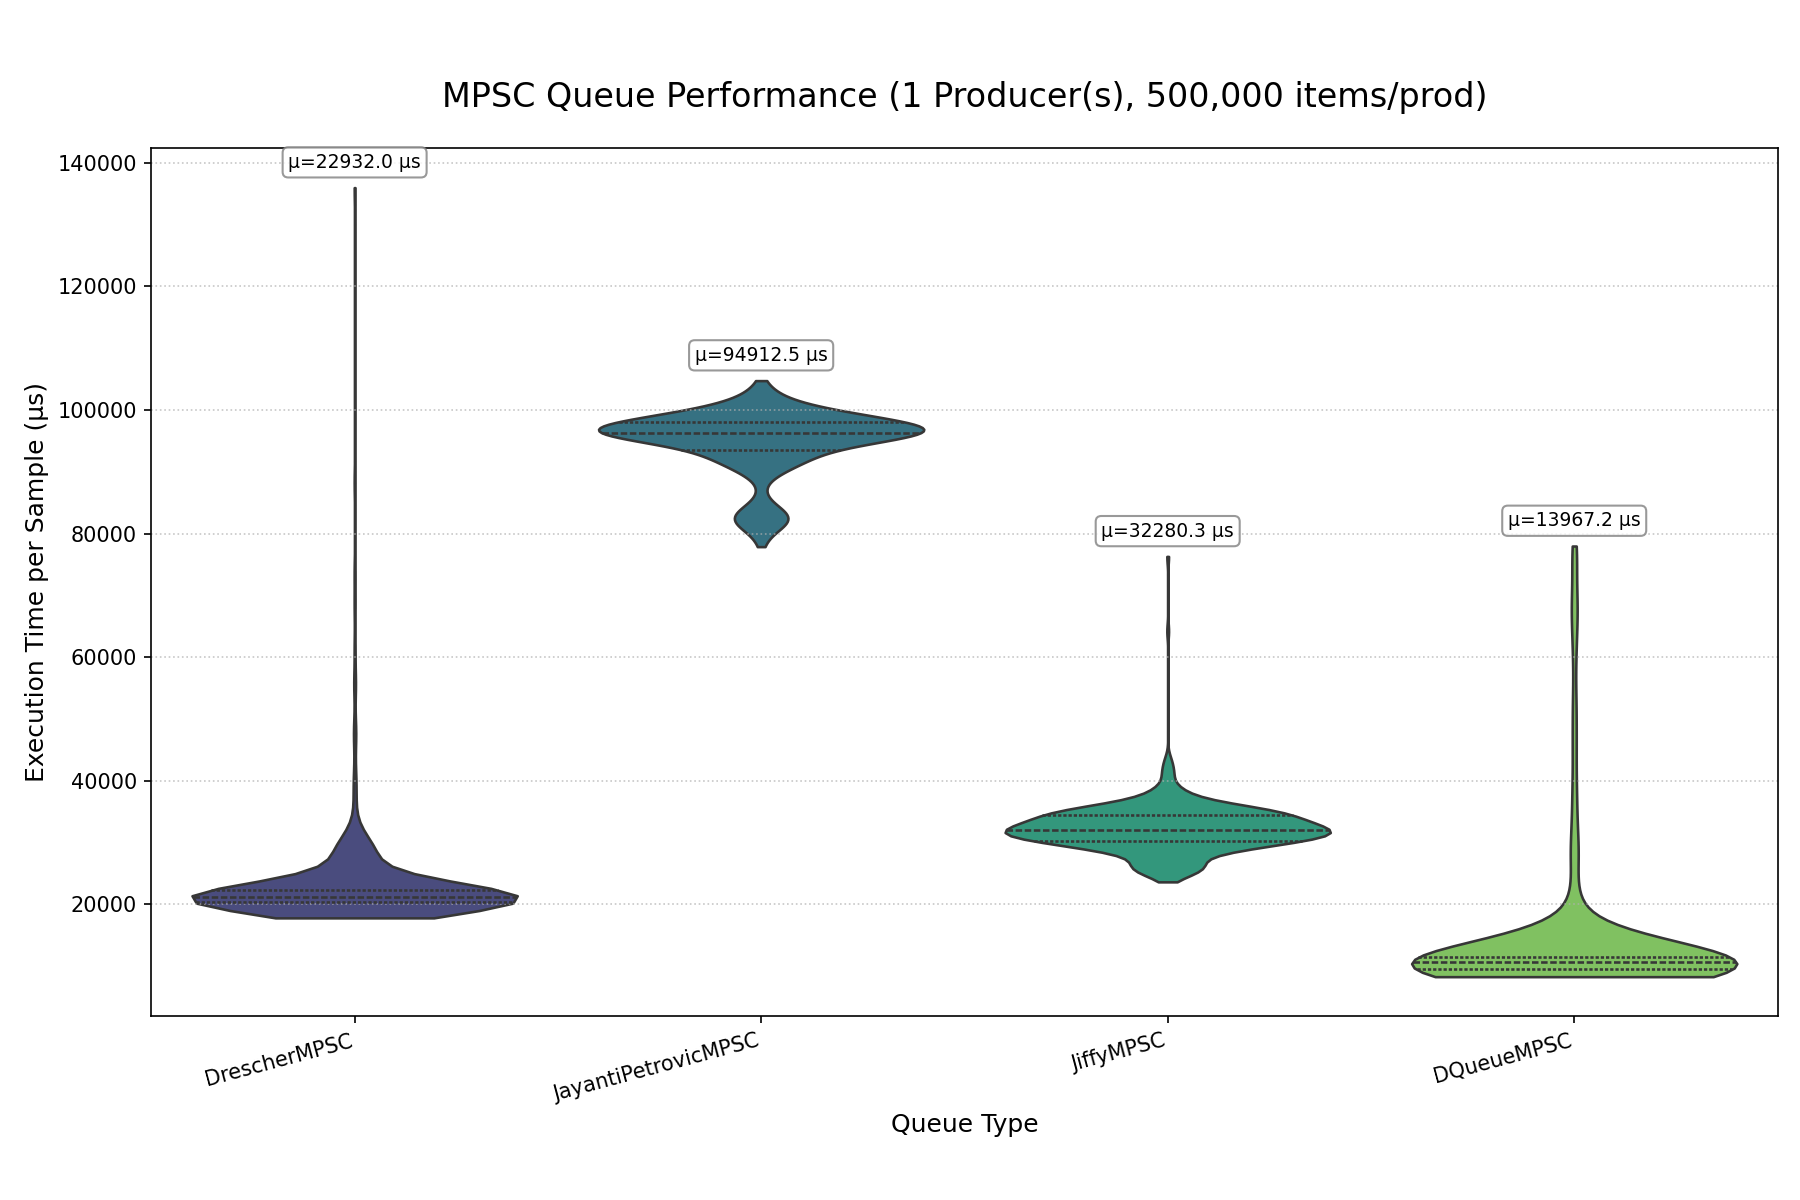
\includegraphics[width=\textwidth]{images/results/mpsc_performance_violin_1_producers.png}
\end{figure}

\begin{figure}[H]
\centering
\caption{MPSC queue performance distribution with 2 producers with 1,000,000 Total Items}
\label{fig:mpsc-violin-2p}
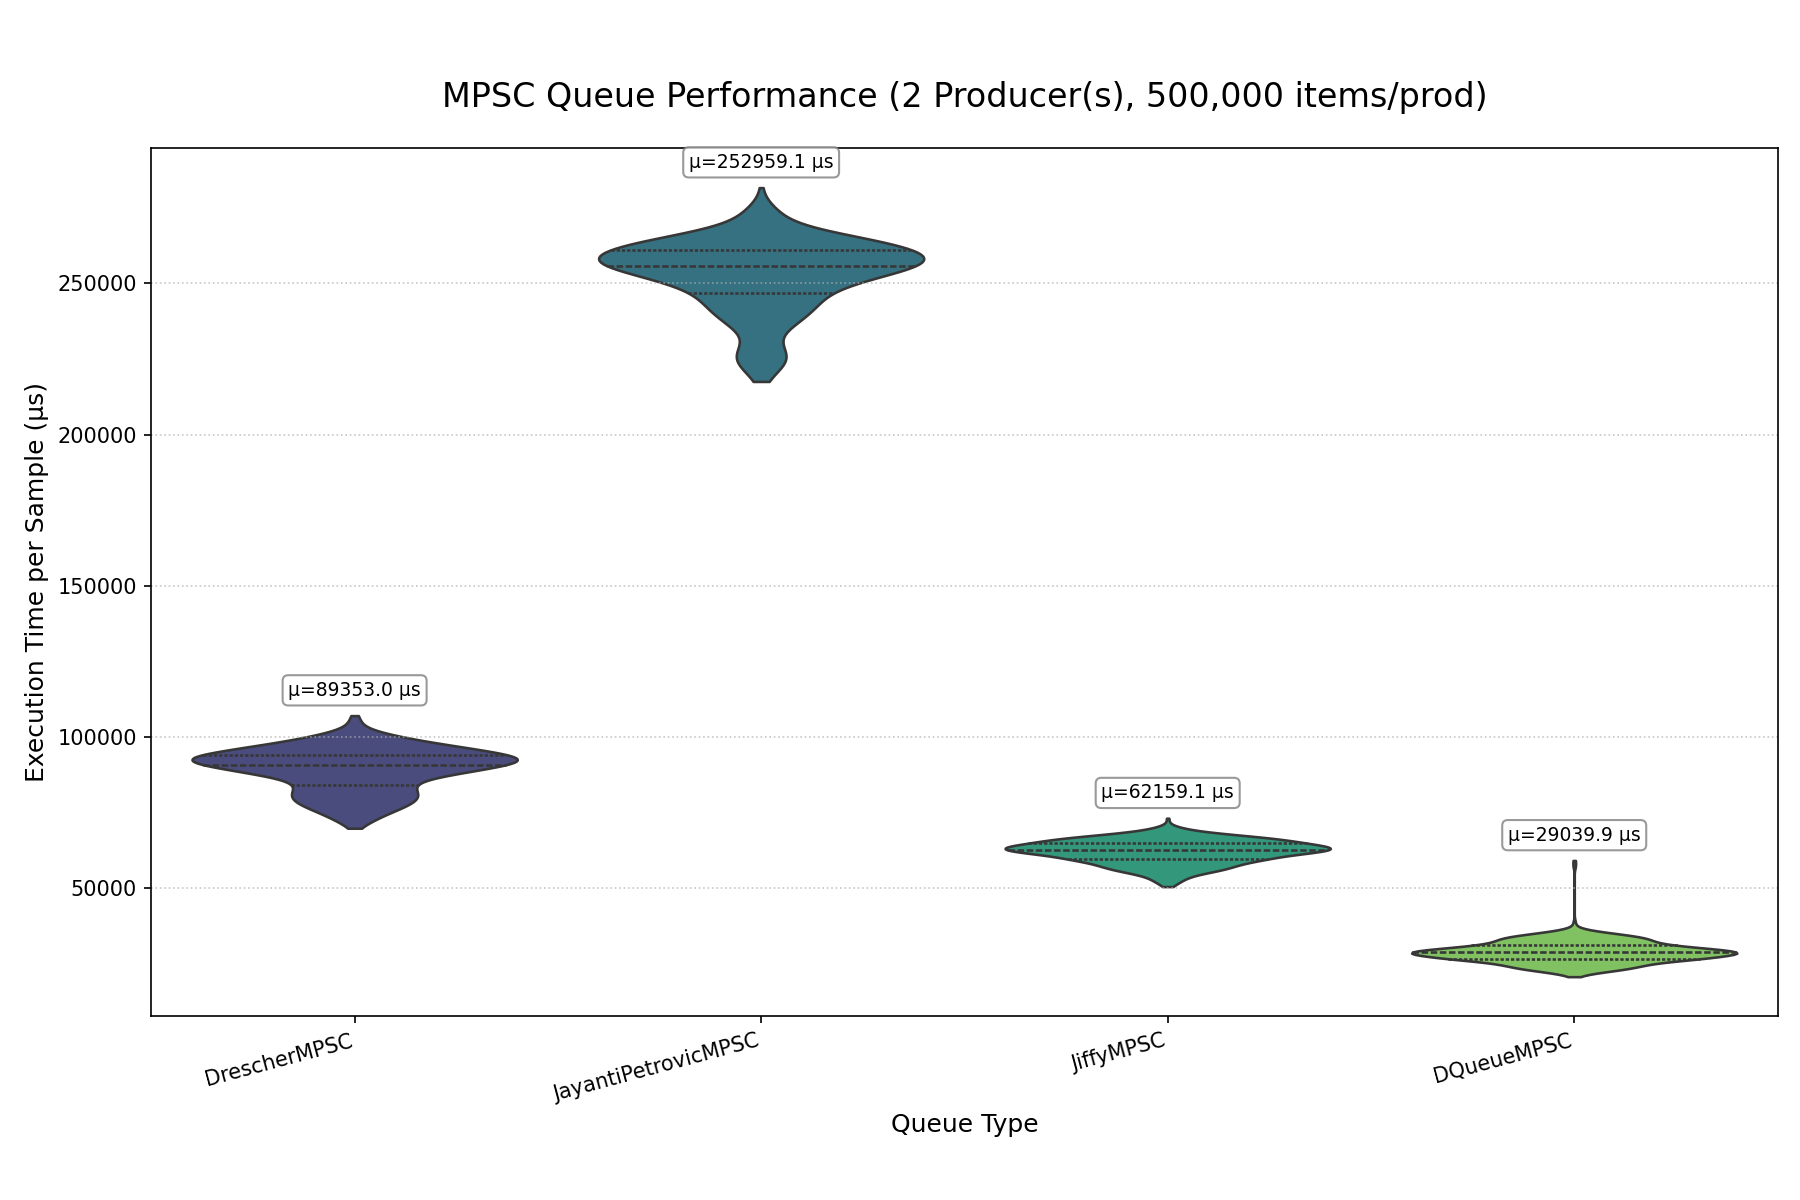
\includegraphics[width=\textwidth]{images/results/mpsc_performance_violin_2_producers.png}
\end{figure}

\begin{figure}[H]
\centering
\caption{MPSC queue performance distribution with 4 producers with 2,000,000 Total Items}
\label{fig:mpsc-violin-4p}
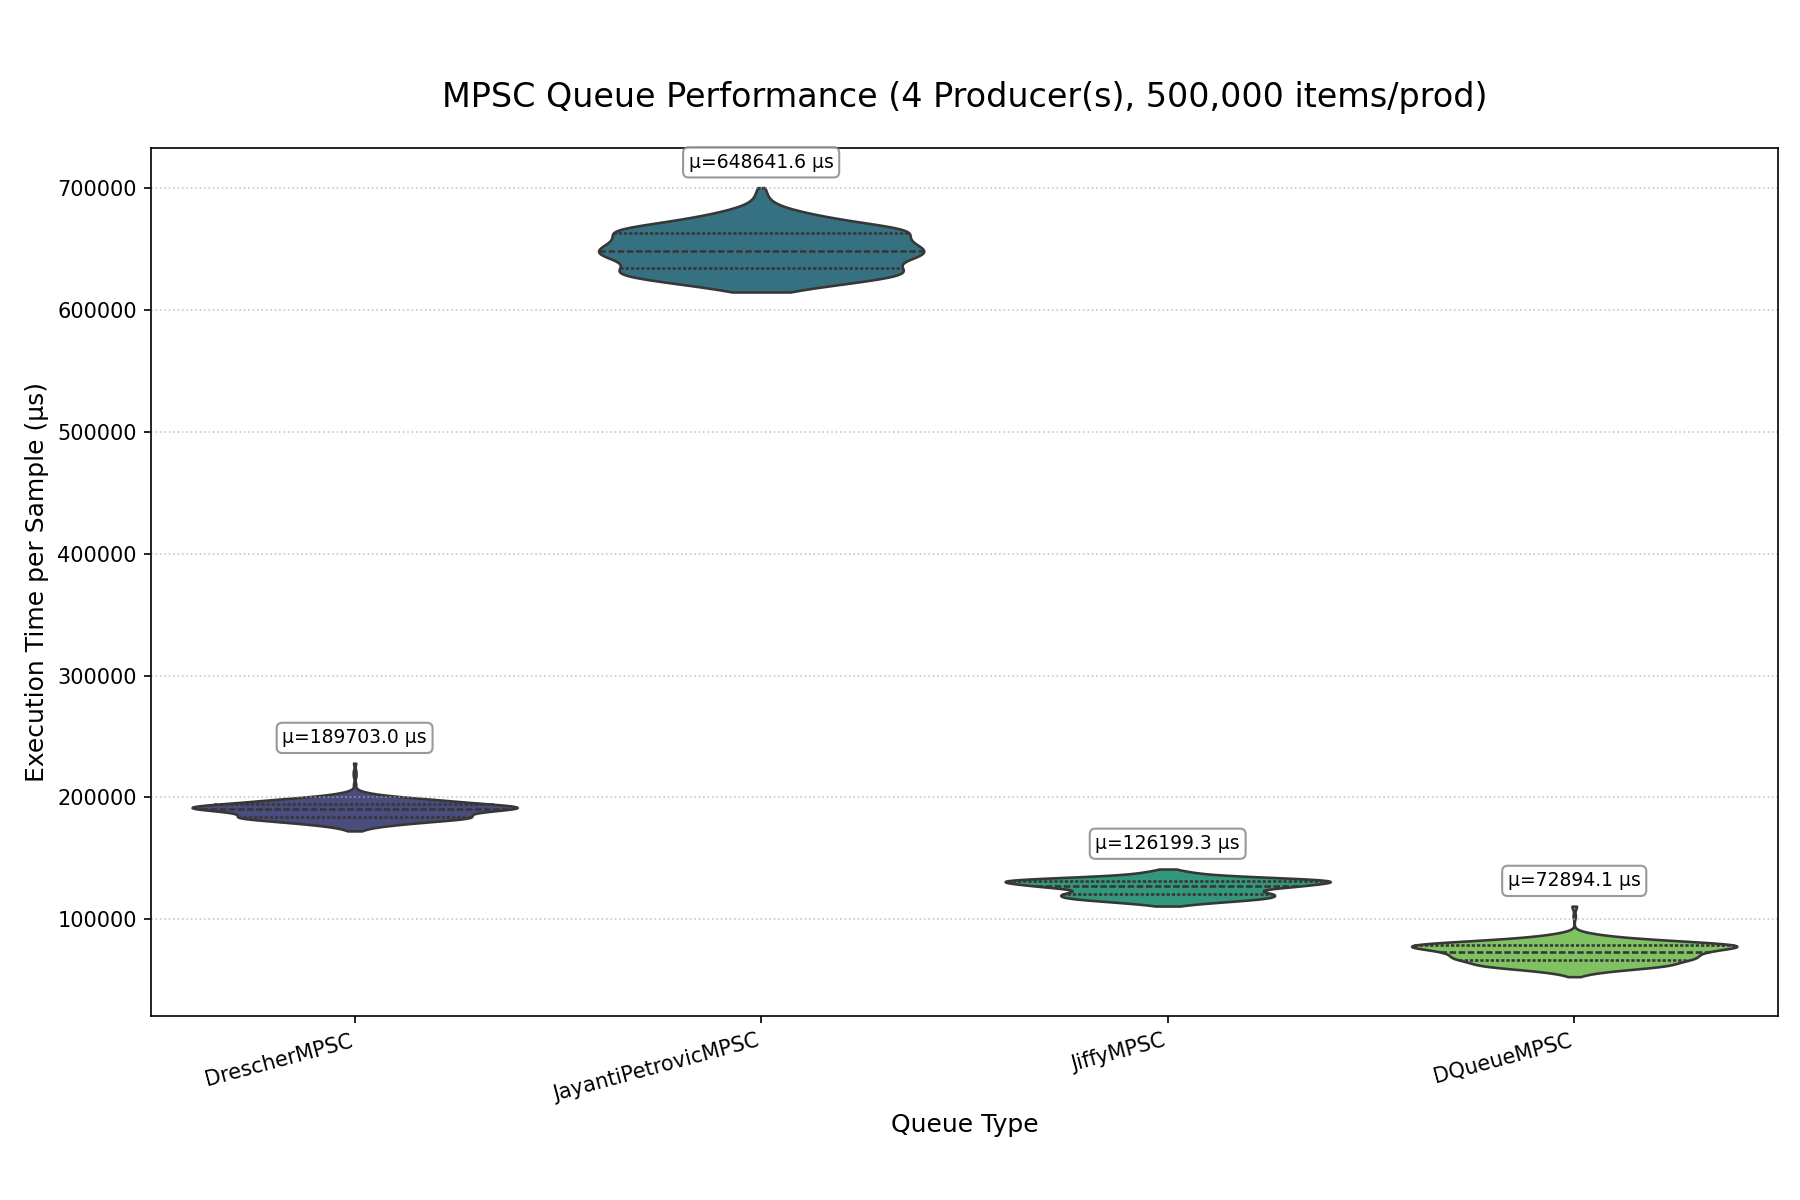
\includegraphics[width=\textwidth]{images/results/mpsc_performance_violin_4_producers.png}
\end{figure}

\begin{figure}[H]
\centering
\caption{MPSC queue performance distribution with 8 producers with 4,000,000 Total Items}
\label{fig:mpsc-violin-8p}
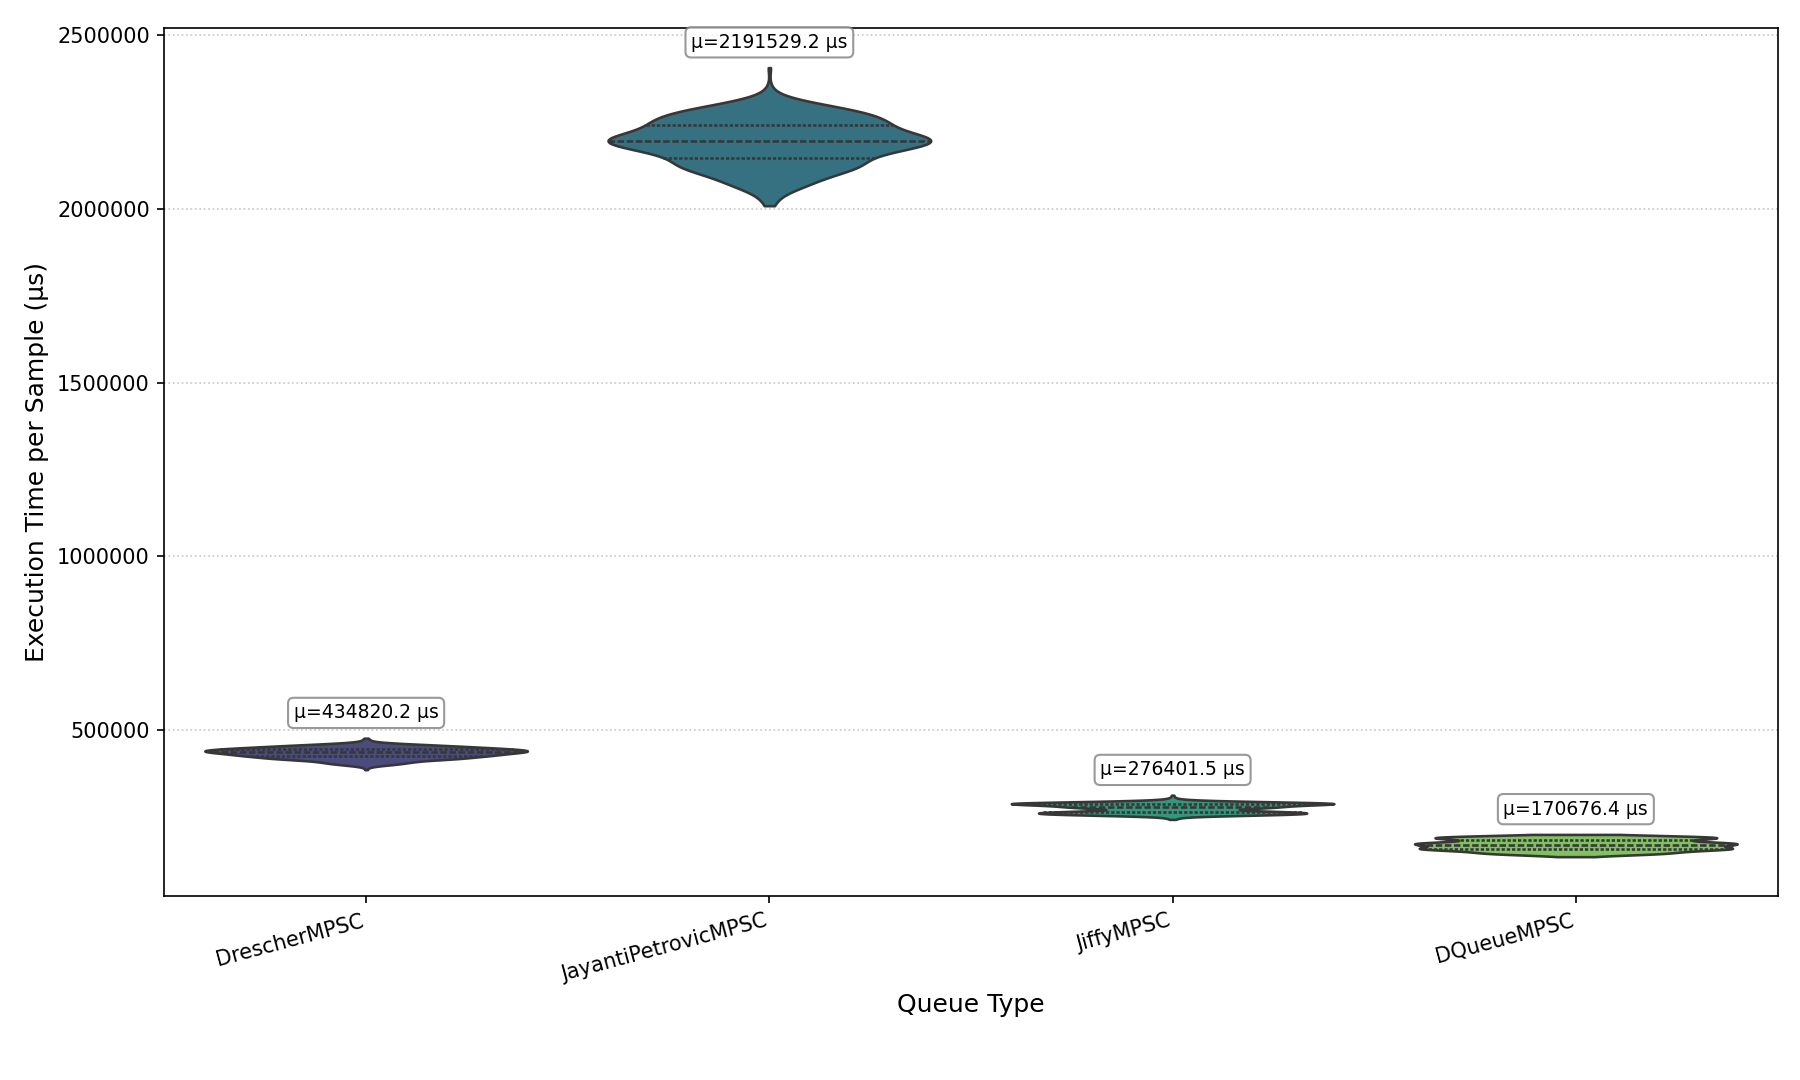
\includegraphics[width=\textwidth]{images/results/mpsc_performance_violin_8_producers.png}
\end{figure}

\subsection{MPMC Queue Performance Distributions}
The following figures show the performance distribution of MPMC queue implementations across different configurations:

\begin{figure}[H]
\centering
\caption{MPMC queue performance distribution with 1 producer and 1 consumer with 170,000 Total Items}
\label{fig:mpmc-violin-1p1c}
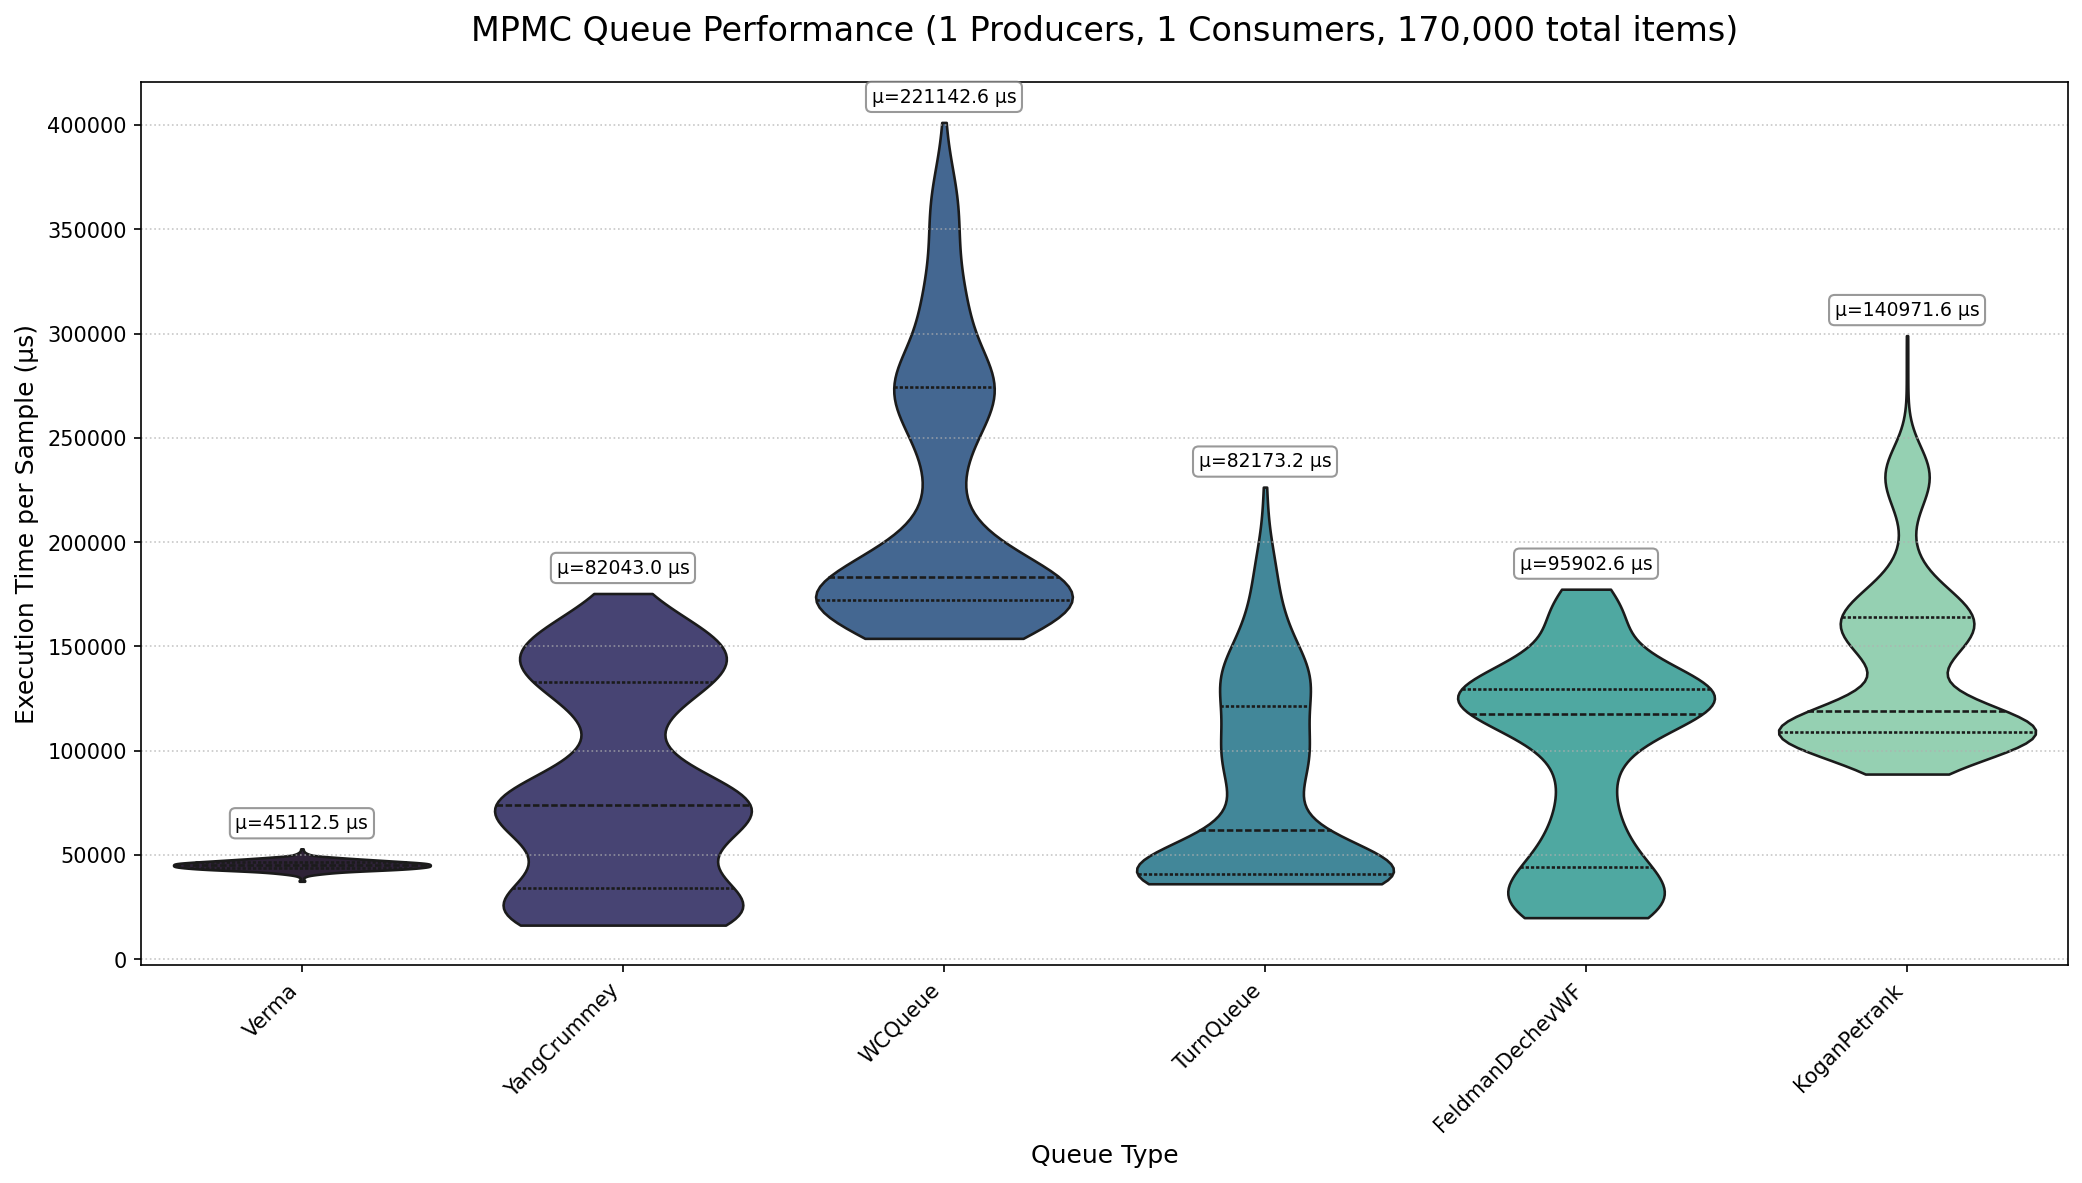
\includegraphics[width=\textwidth]{images/results/mpmc_performance_violin_1P_1C.png}
\end{figure}

\begin{figure}[H]
\centering
\caption{MPMC queue performance distribution with 2 producers and 2 consumers with 340,000 Total Items}
\label{fig:mpmc-violin-2p2c}
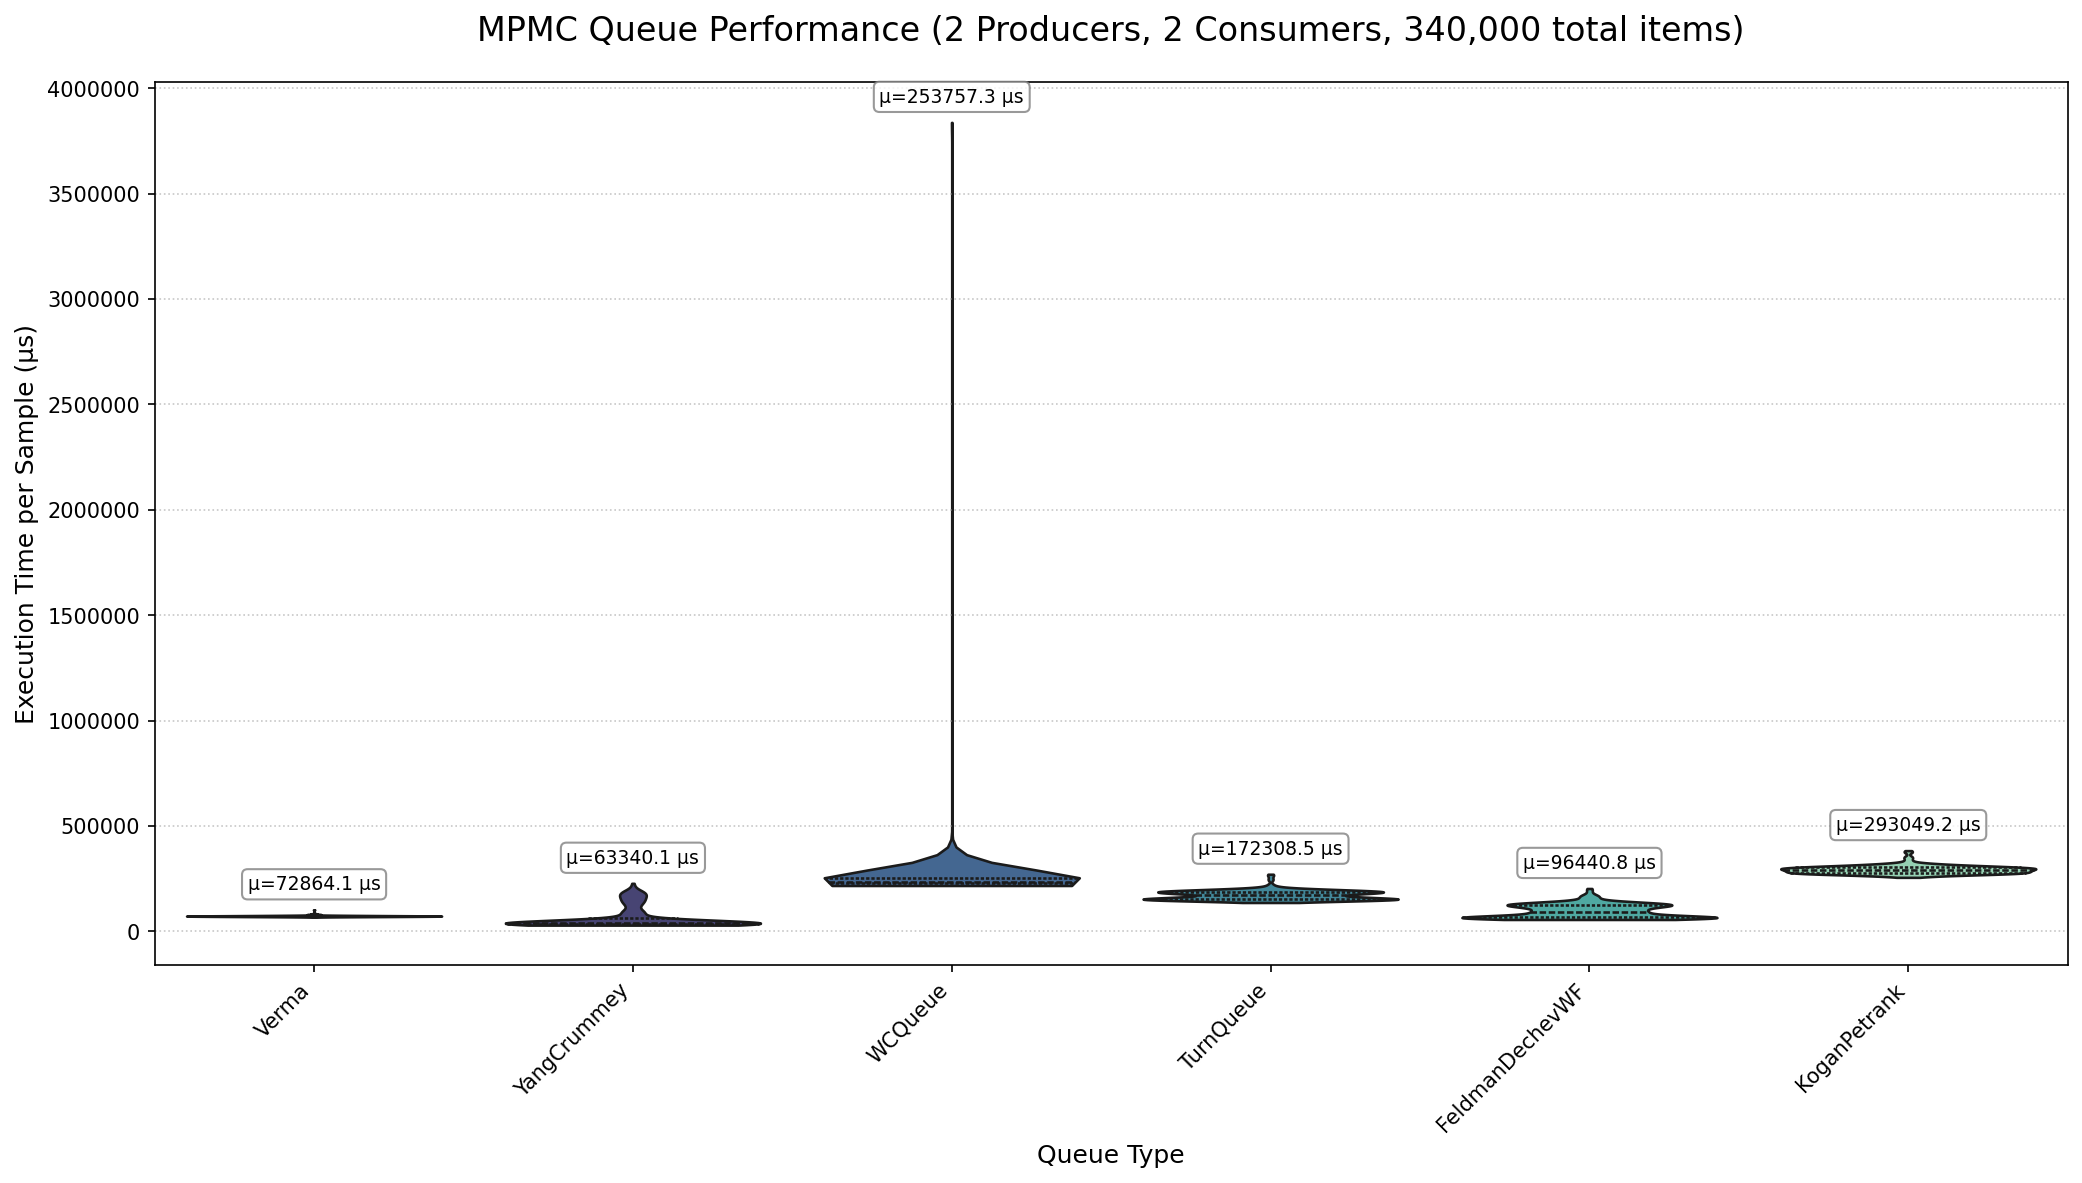
\includegraphics[width=\textwidth]{images/results/mpmc_performance_violin_2P_2C.png}
\end{figure}

\begin{figure}[H]
\centering
\caption{MPMC queue performance distribution with 4 producers and 4 consumers with 680,000 Total Items}
\label{fig:mpmc-violin-4p4c}
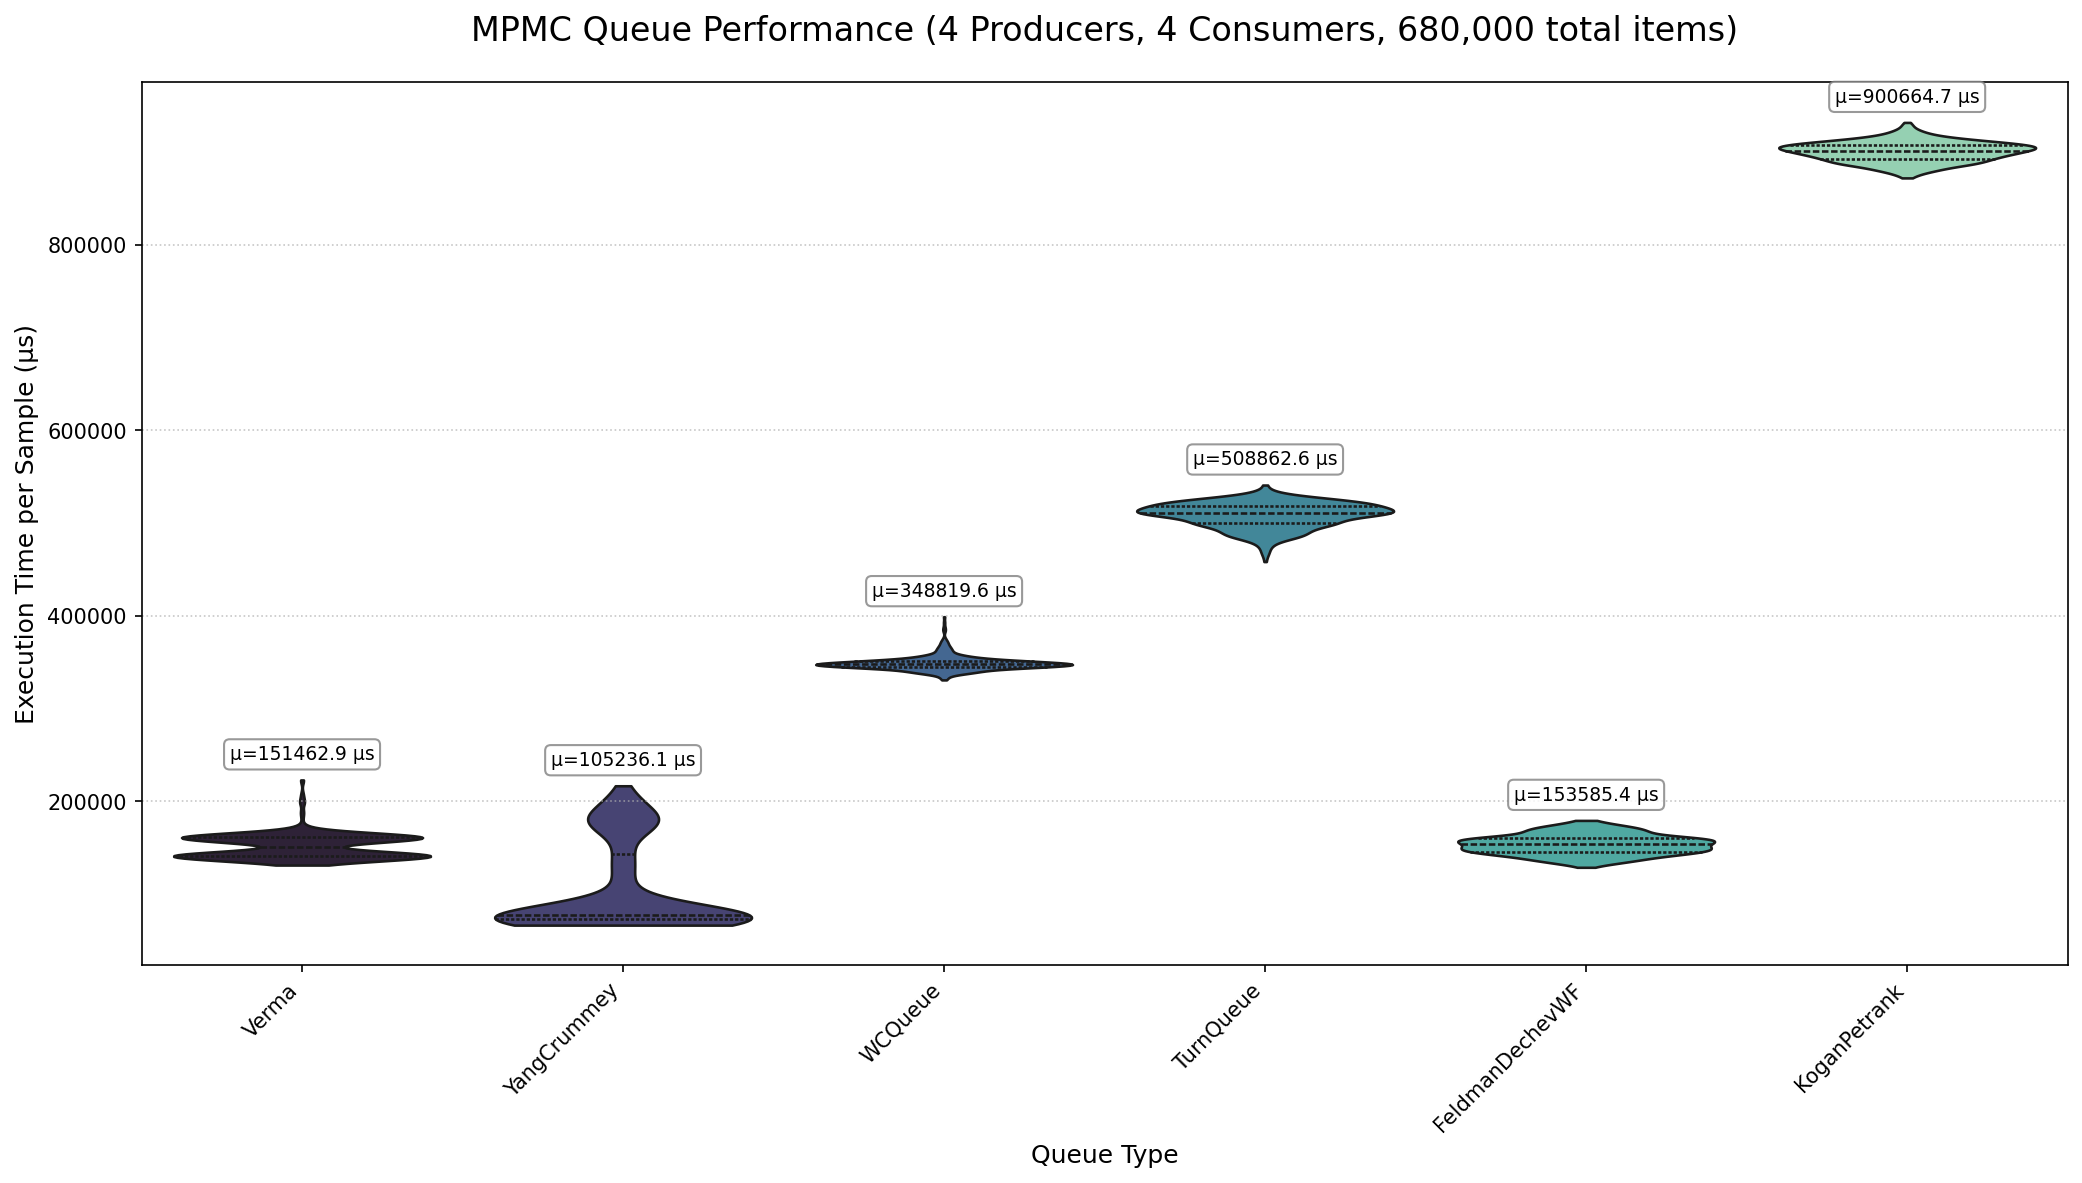
\includegraphics[width=\textwidth]{images/results/mpmc_performance_violin_4P_4C.png}
\end{figure}

\subsection{Cross-Category Performance Distributions}
The following figures show performance distributions when queues from different categories operate in various contention scenarios:

\subsubsection{Cross-Category MPSC Performance}
\begin{figure}[H]
\centering
\caption{Cross-category MPSC performance distribution with 1 producer and 1 consumer with 100,000 Total Items}
\label{fig:cross-mpsc-violin-1p}
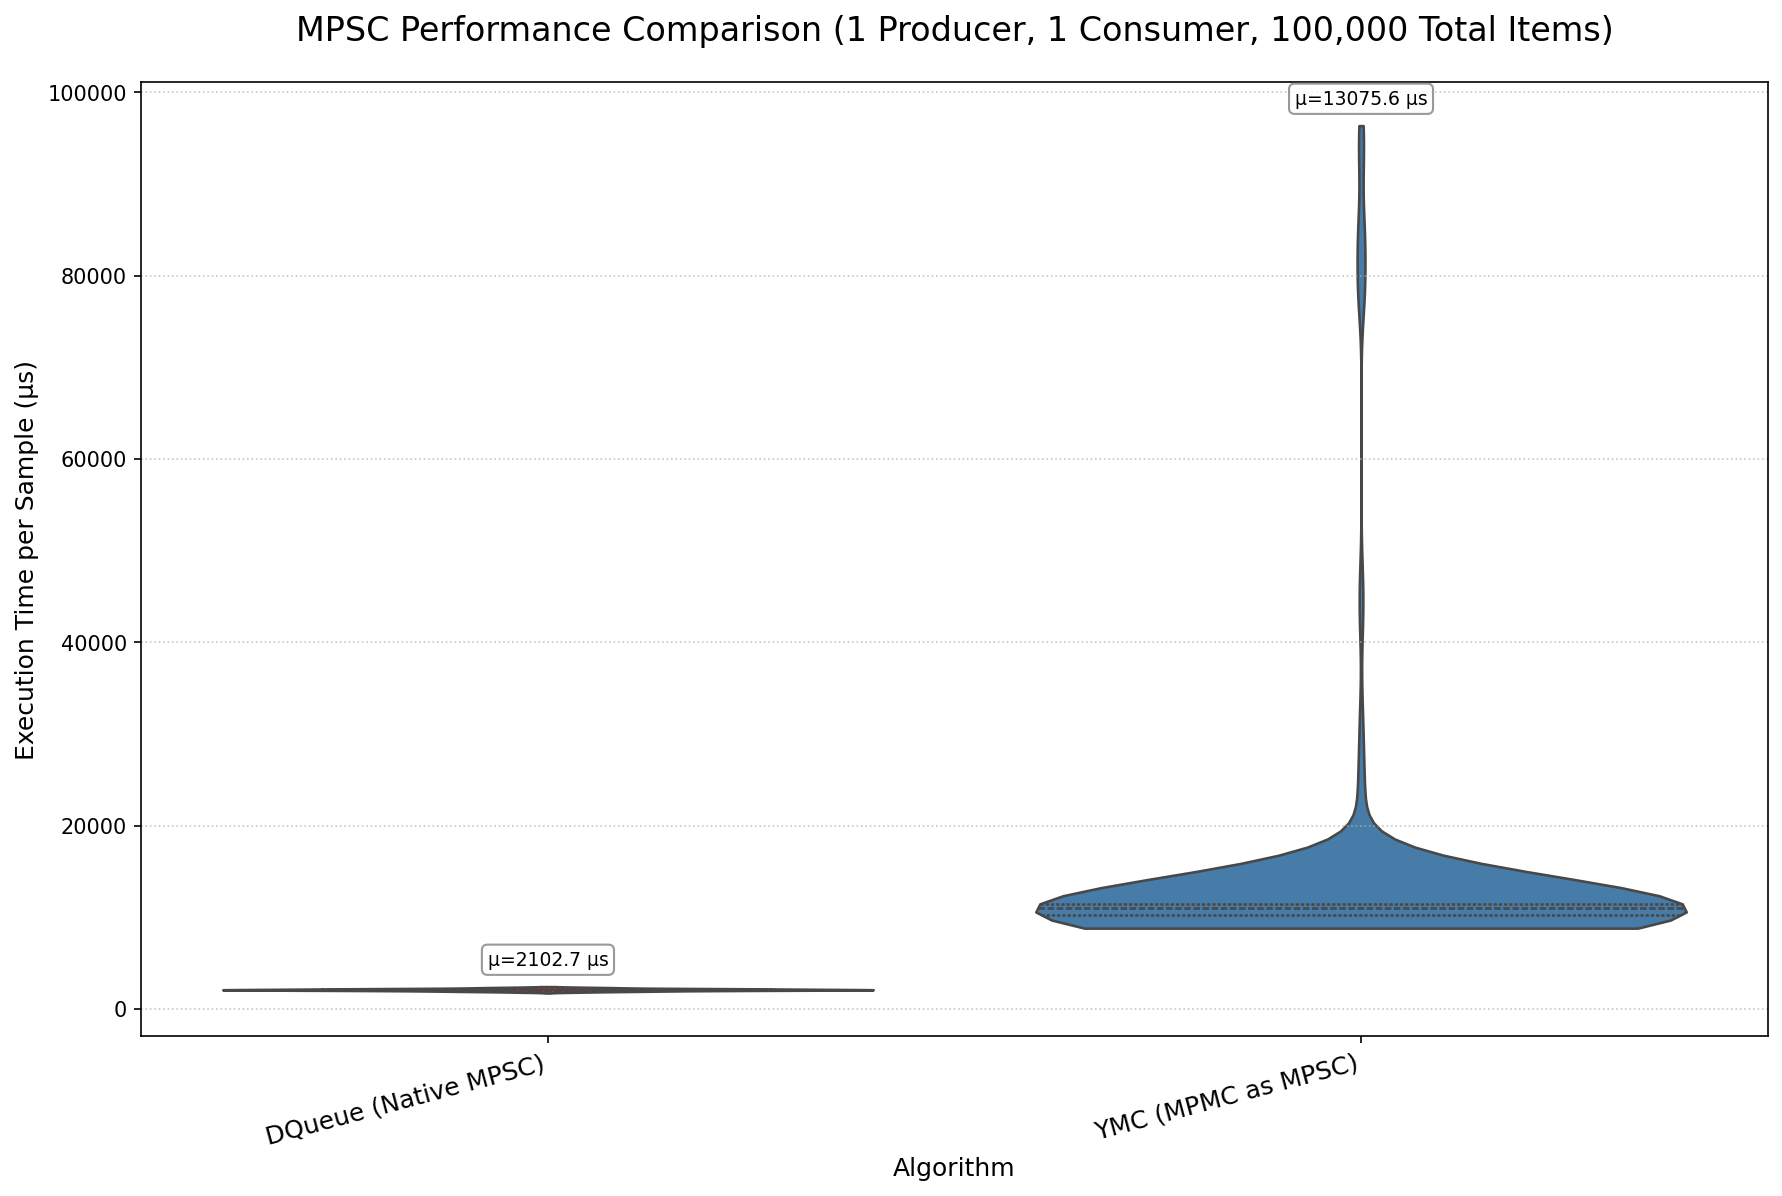
\includegraphics[width=\textwidth]{images/results/best_in_mpsc_performance_violin_1P1C.png}
\end{figure}

\begin{figure}[H]
\centering
\caption{Cross-category MPSC performance distribution with 2 producers and 1 consumer with 200,000 Total Items}
\label{fig:cross-mpsc-violin-2p}
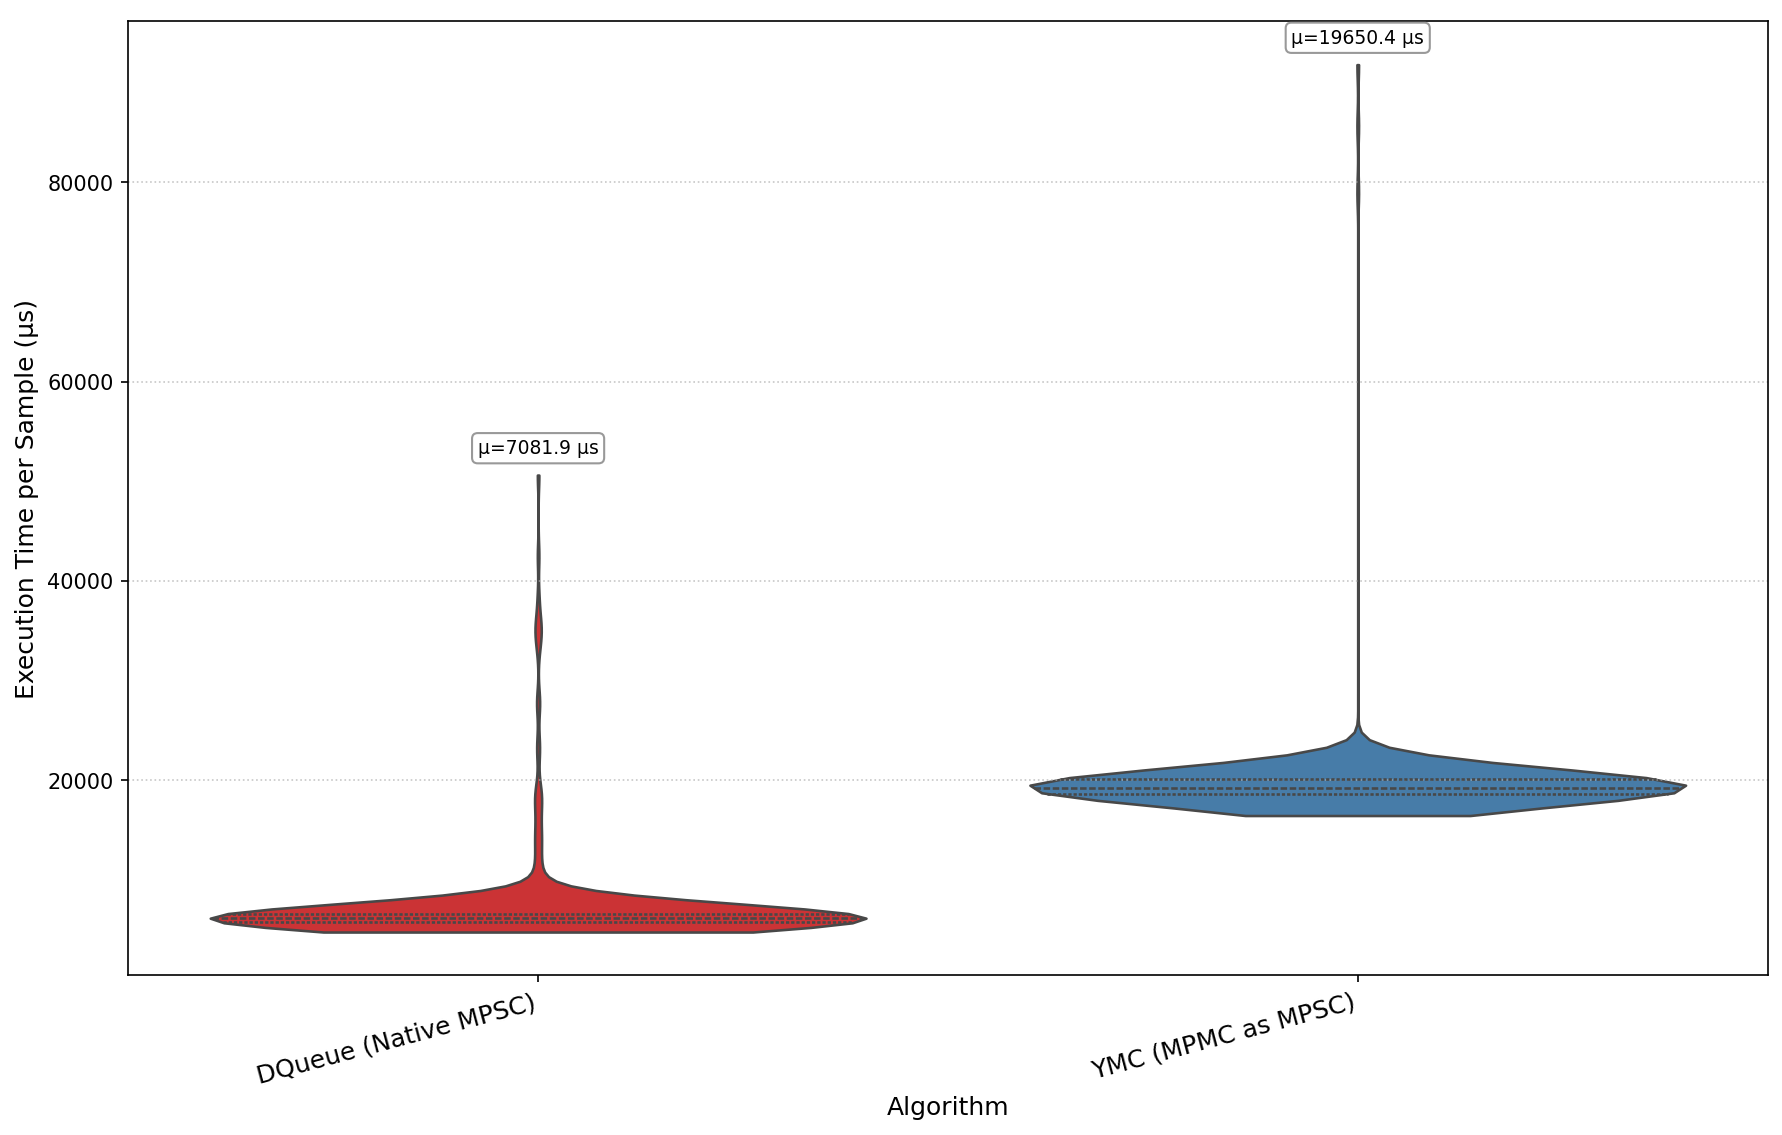
\includegraphics[width=\textwidth]{images/results/best_in_mpsc_performance_violin_2P1C.png}
\end{figure}

\begin{figure}[H]
\centering
\caption{Cross-category MPSC performance distribution with 4 producers and 1 consumer with 400,000 Total Items}
\label{fig:cross-mpsc-violin-4p}
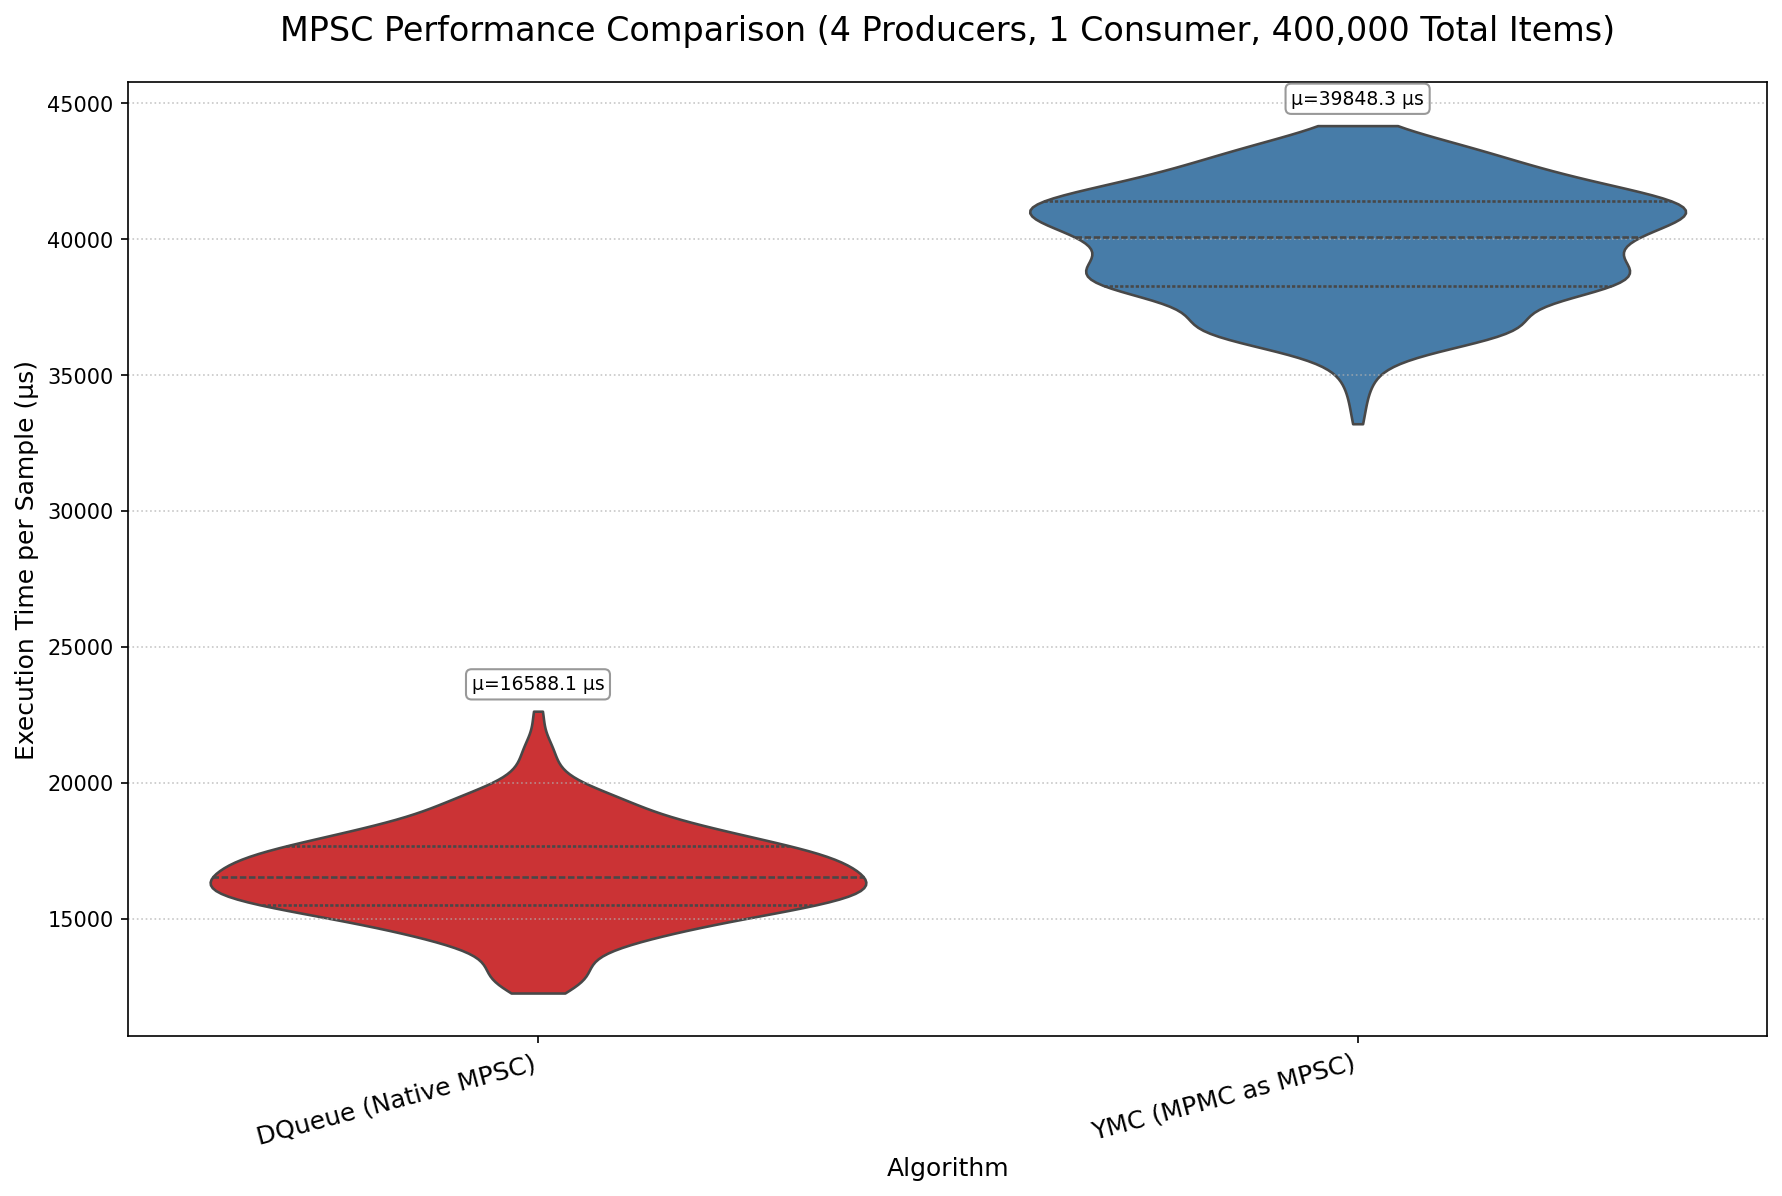
\includegraphics[width=\textwidth]{images/results/best_in_mpsc_performance_violin_4P1C.png}
\end{figure}

\begin{figure}[H]
\centering
\caption{Cross-category MPSC performance distribution with 8 producers and 1 consumer with 800,000 Total Items}
\label{fig:cross-mpsc-violin-8p}
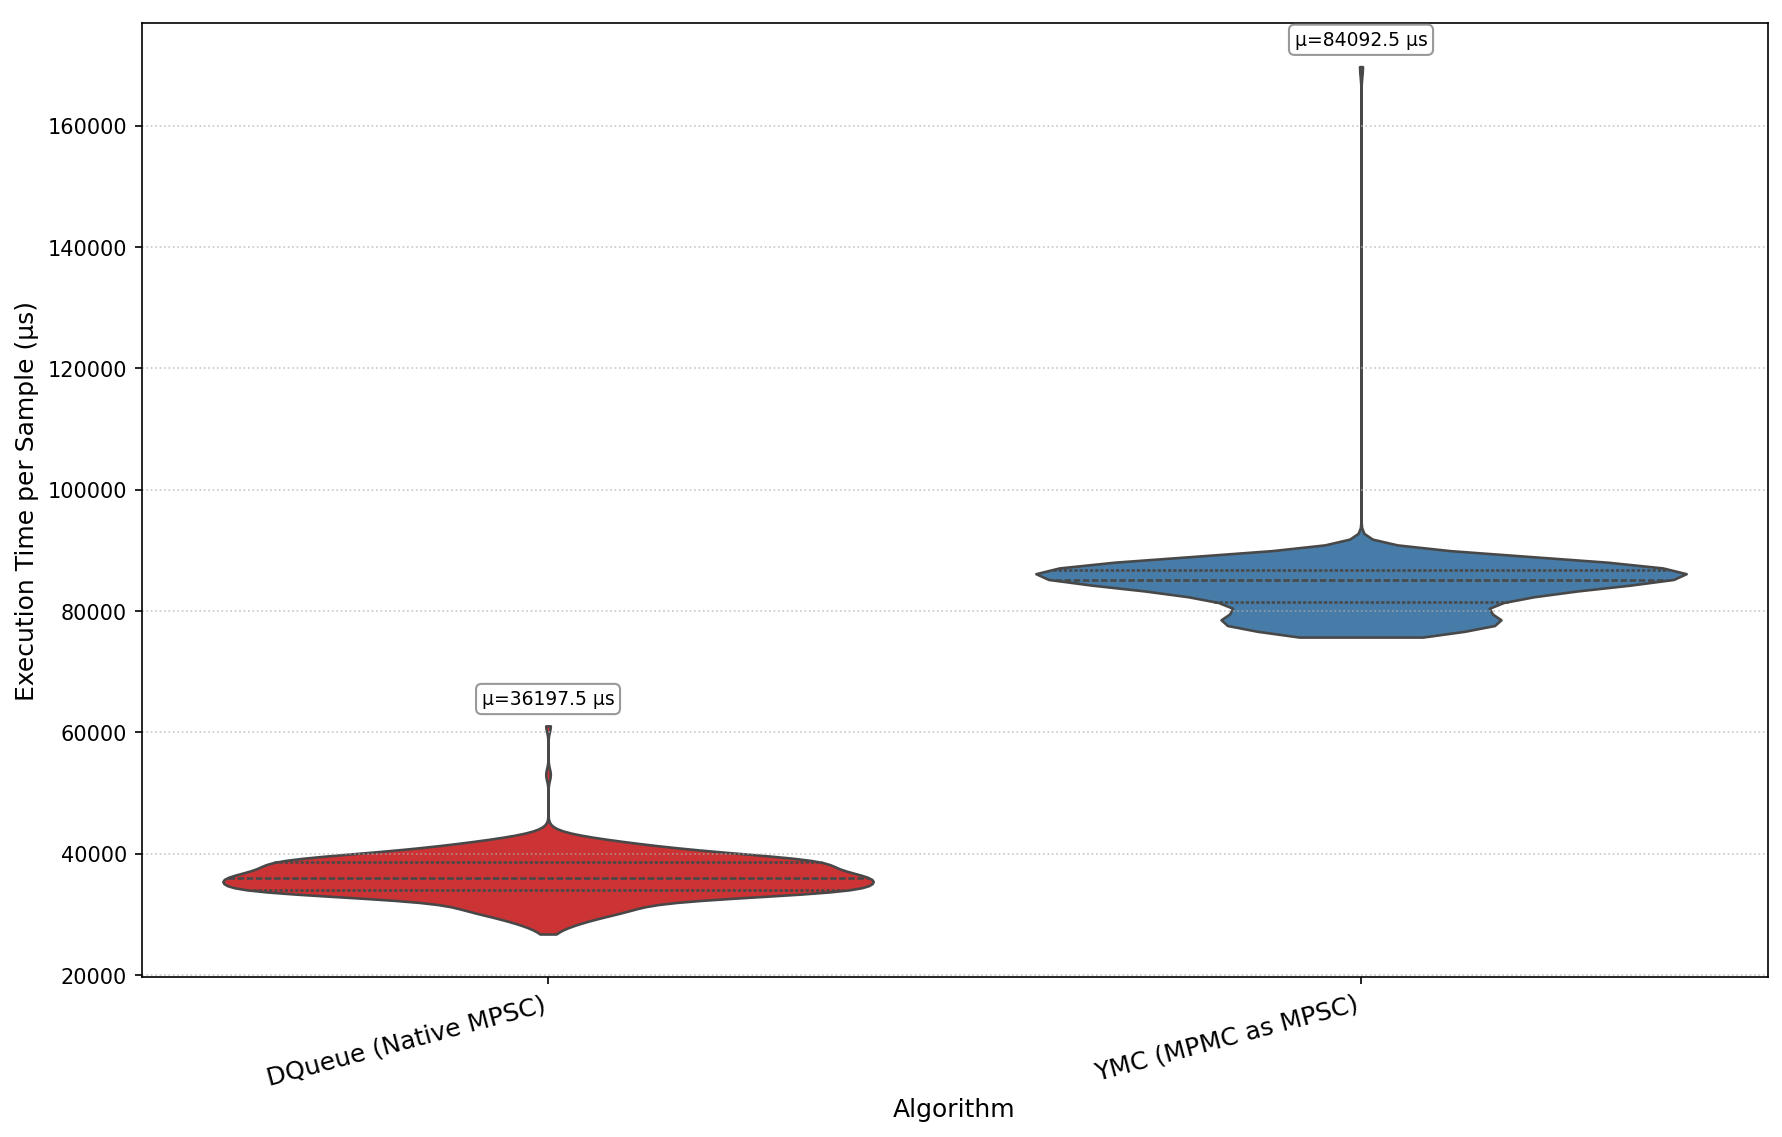
\includegraphics[width=\textwidth]{images/results/best_in_mpsc_performance_violin_8P1C.png}
\end{figure}

\subsubsection{Cross-Category SPMC Performance}
\begin{figure}[H]
\centering
\caption{Cross-category SPMC performance distribution with 1 producer and 1 consumer with 100,000 Total Items}
\label{fig:cross-spmc-violin-1c}
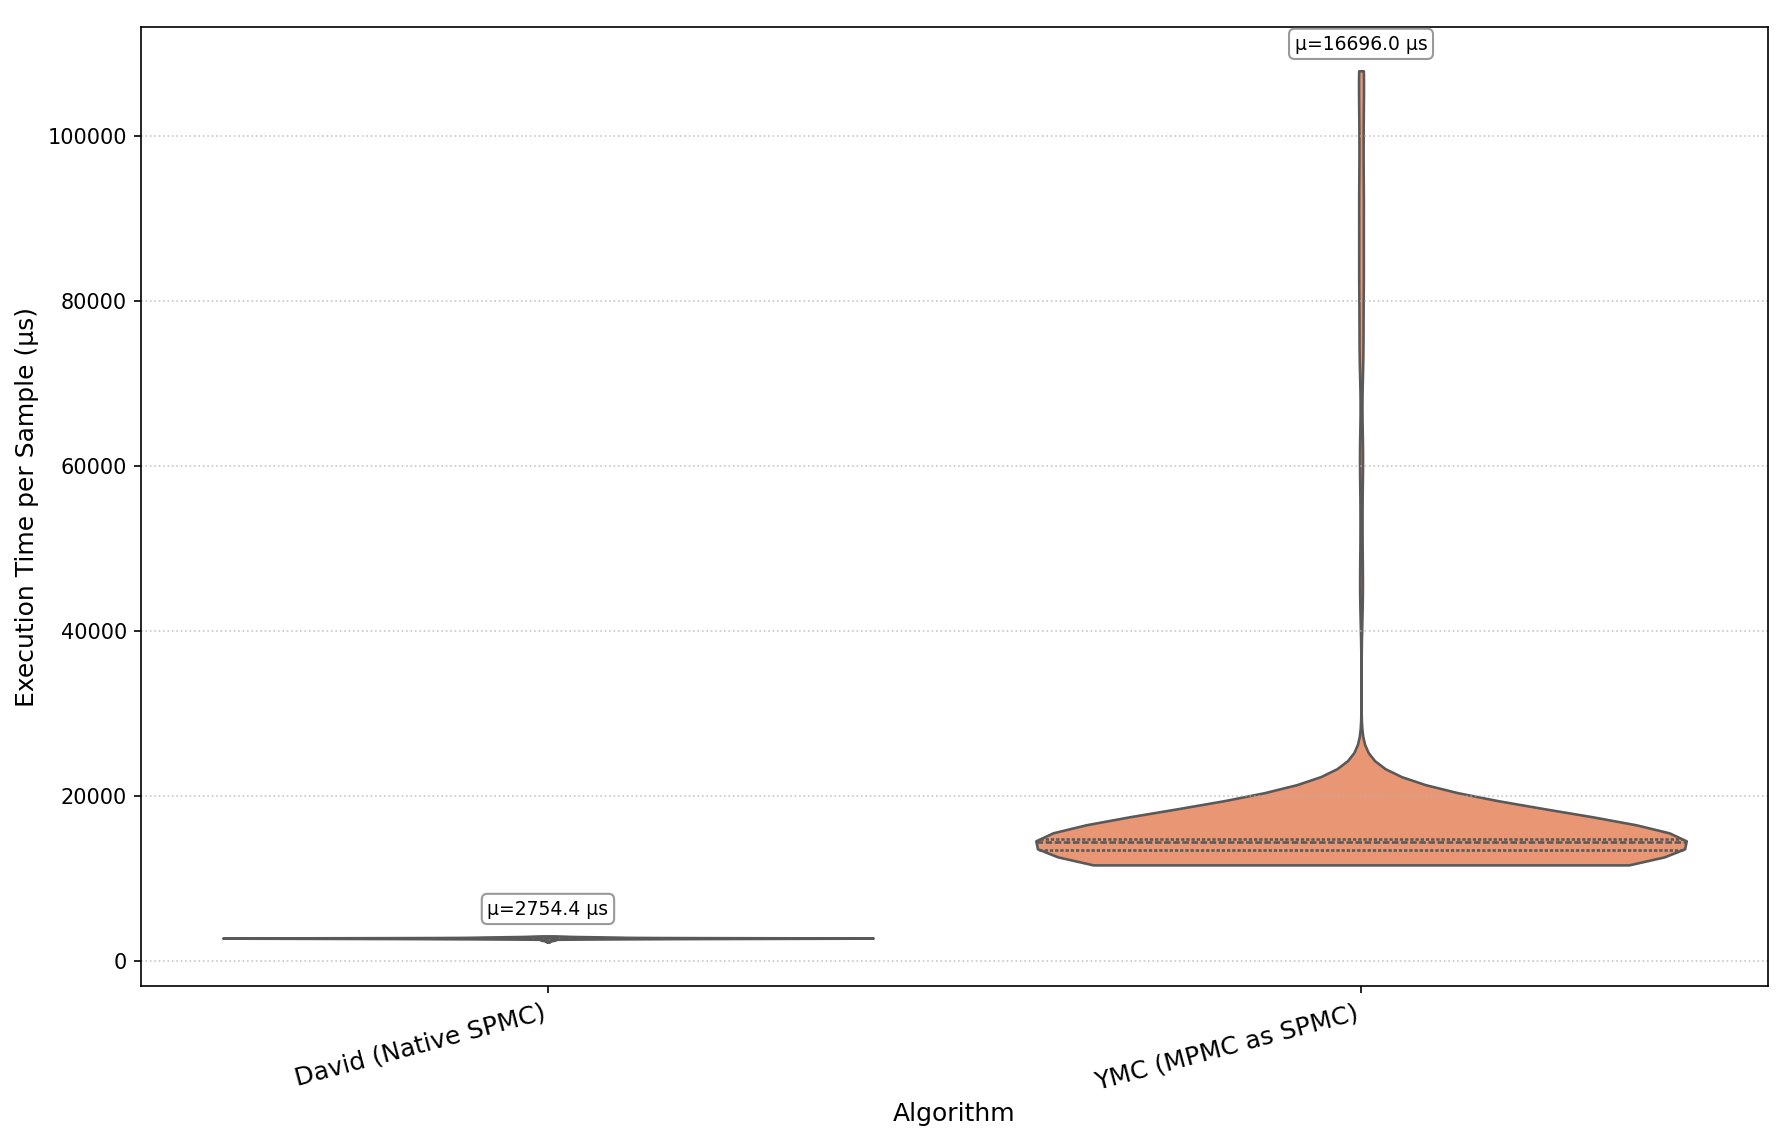
\includegraphics[width=\textwidth]{images/results/best_in_spmc_performance_violin_1P1C.png}
\end{figure}

\begin{figure}[H]
\centering
\caption{Cross-category SPMC performance distribution with 1 producer and 2 consumers with 200,000 Total Items}
\label{fig:cross-spmc-violin-2c}
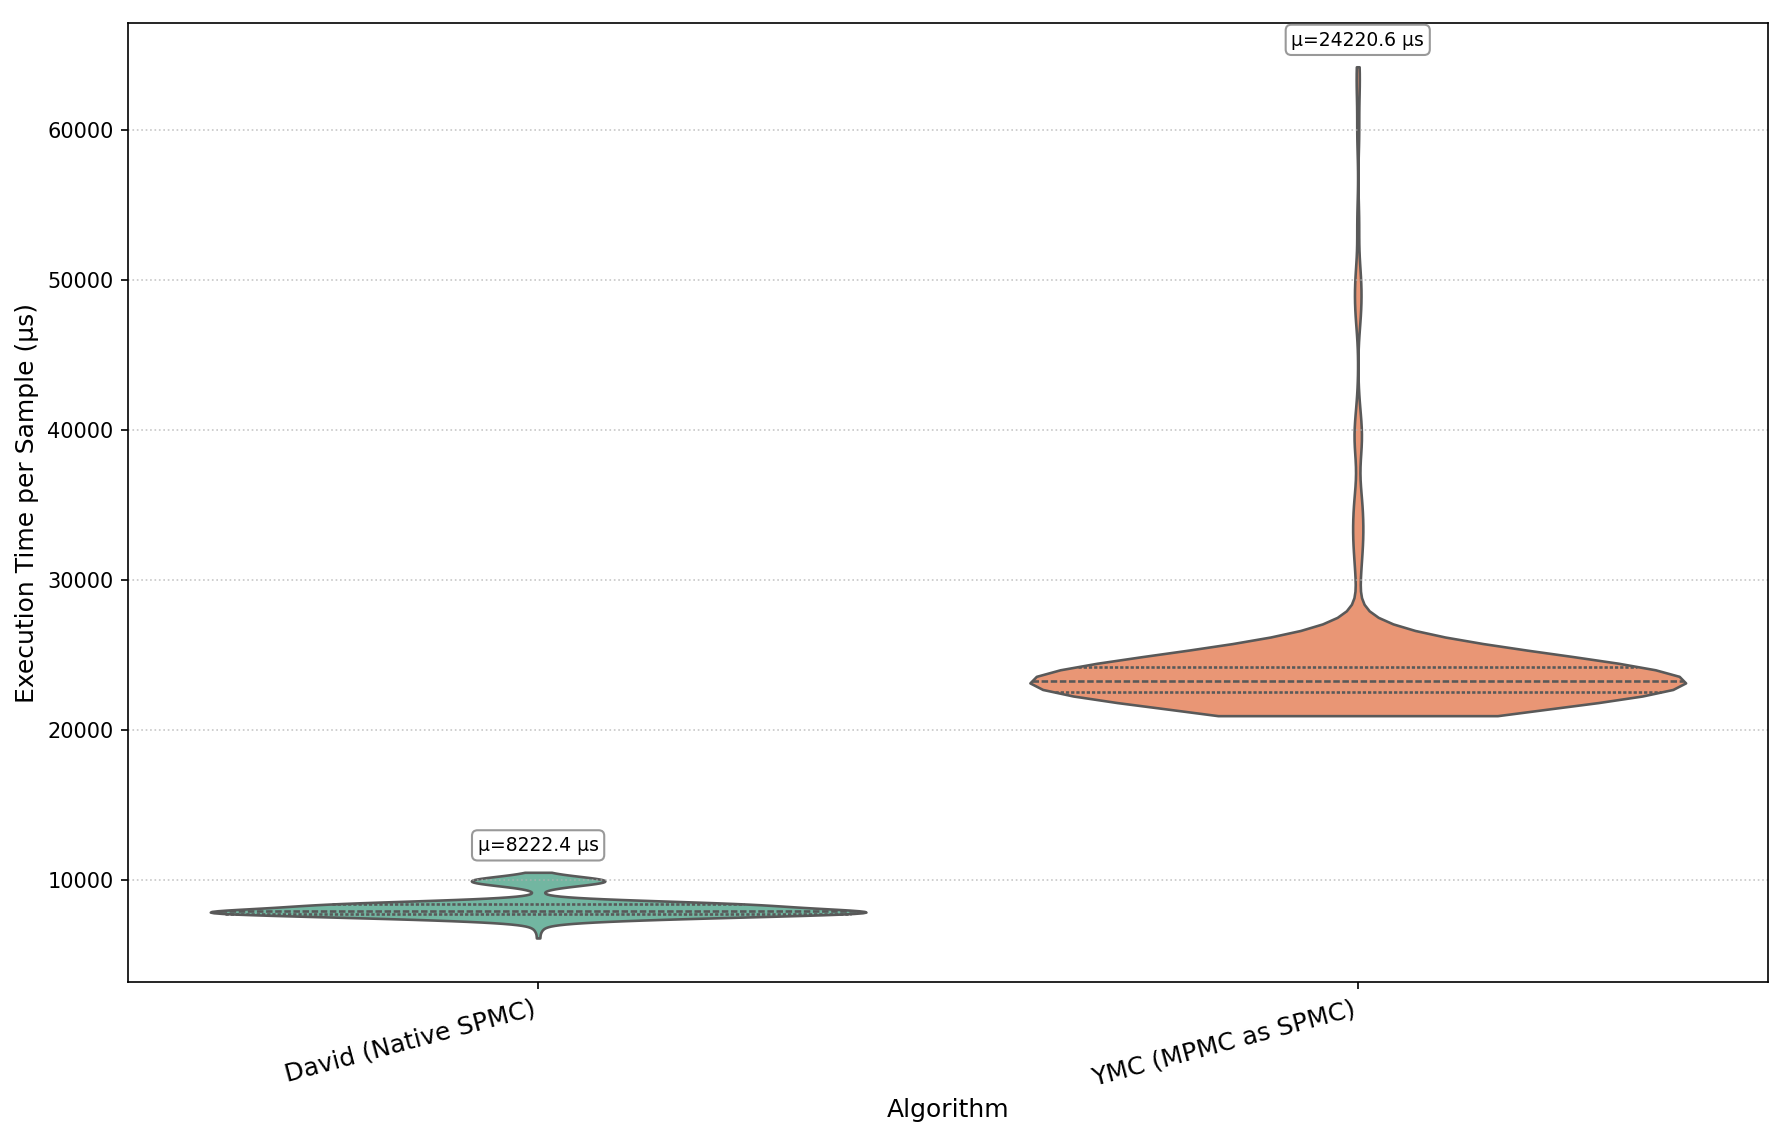
\includegraphics[width=\textwidth]{images/results/best_in_spmc_performance_violin_1P2C.png}
\end{figure}

\begin{figure}[H]
\centering
\caption{Cross-category SPMC performance distribution with 1 producer and 4 consumers with 400,000 Total Items}
\label{fig:cross-spmc-violin-4c}
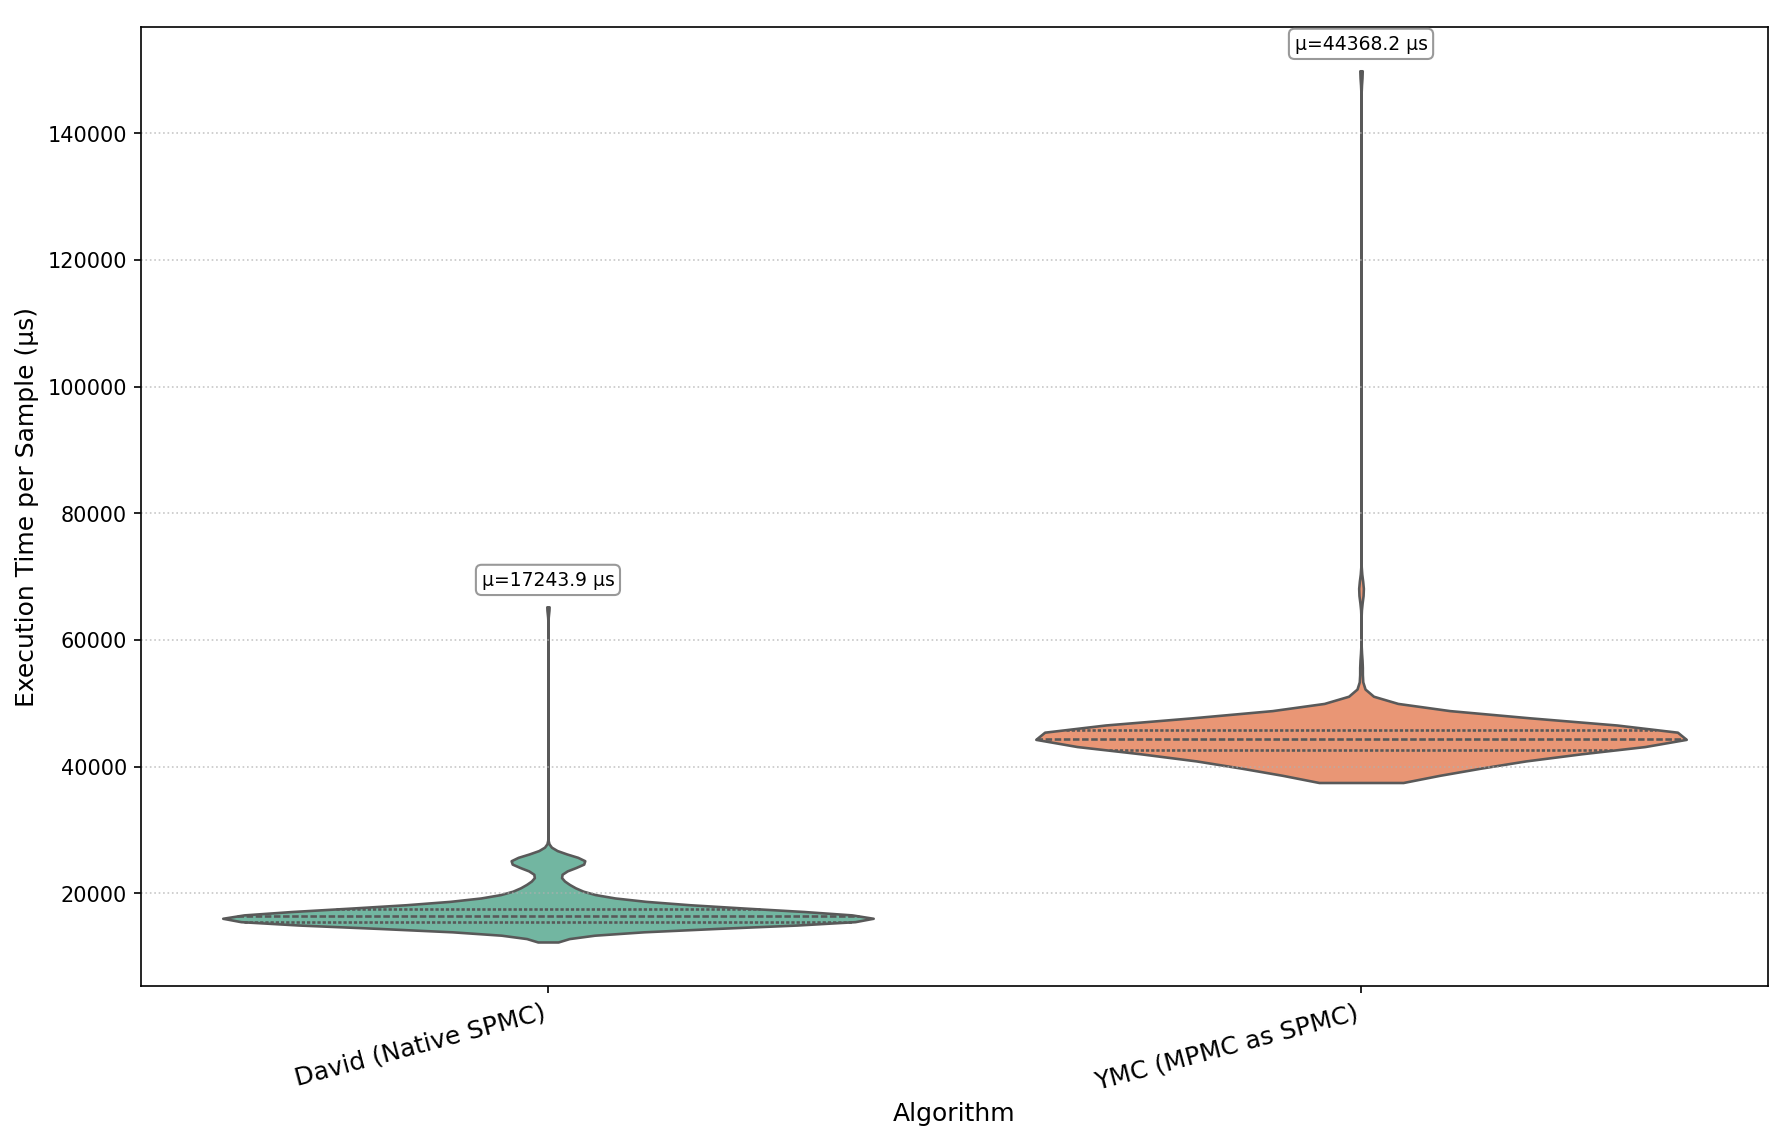
\includegraphics[width=\textwidth]{images/results/best_in_spmc_performance_violin_1P4C.png}
\end{figure}

\begin{figure}[H]
\centering
\caption{Cross-category SPMC performance distribution with 1 producer and 8 consumers with 800,000 Total Items}
\label{fig:cross-spmc-violin-8c}
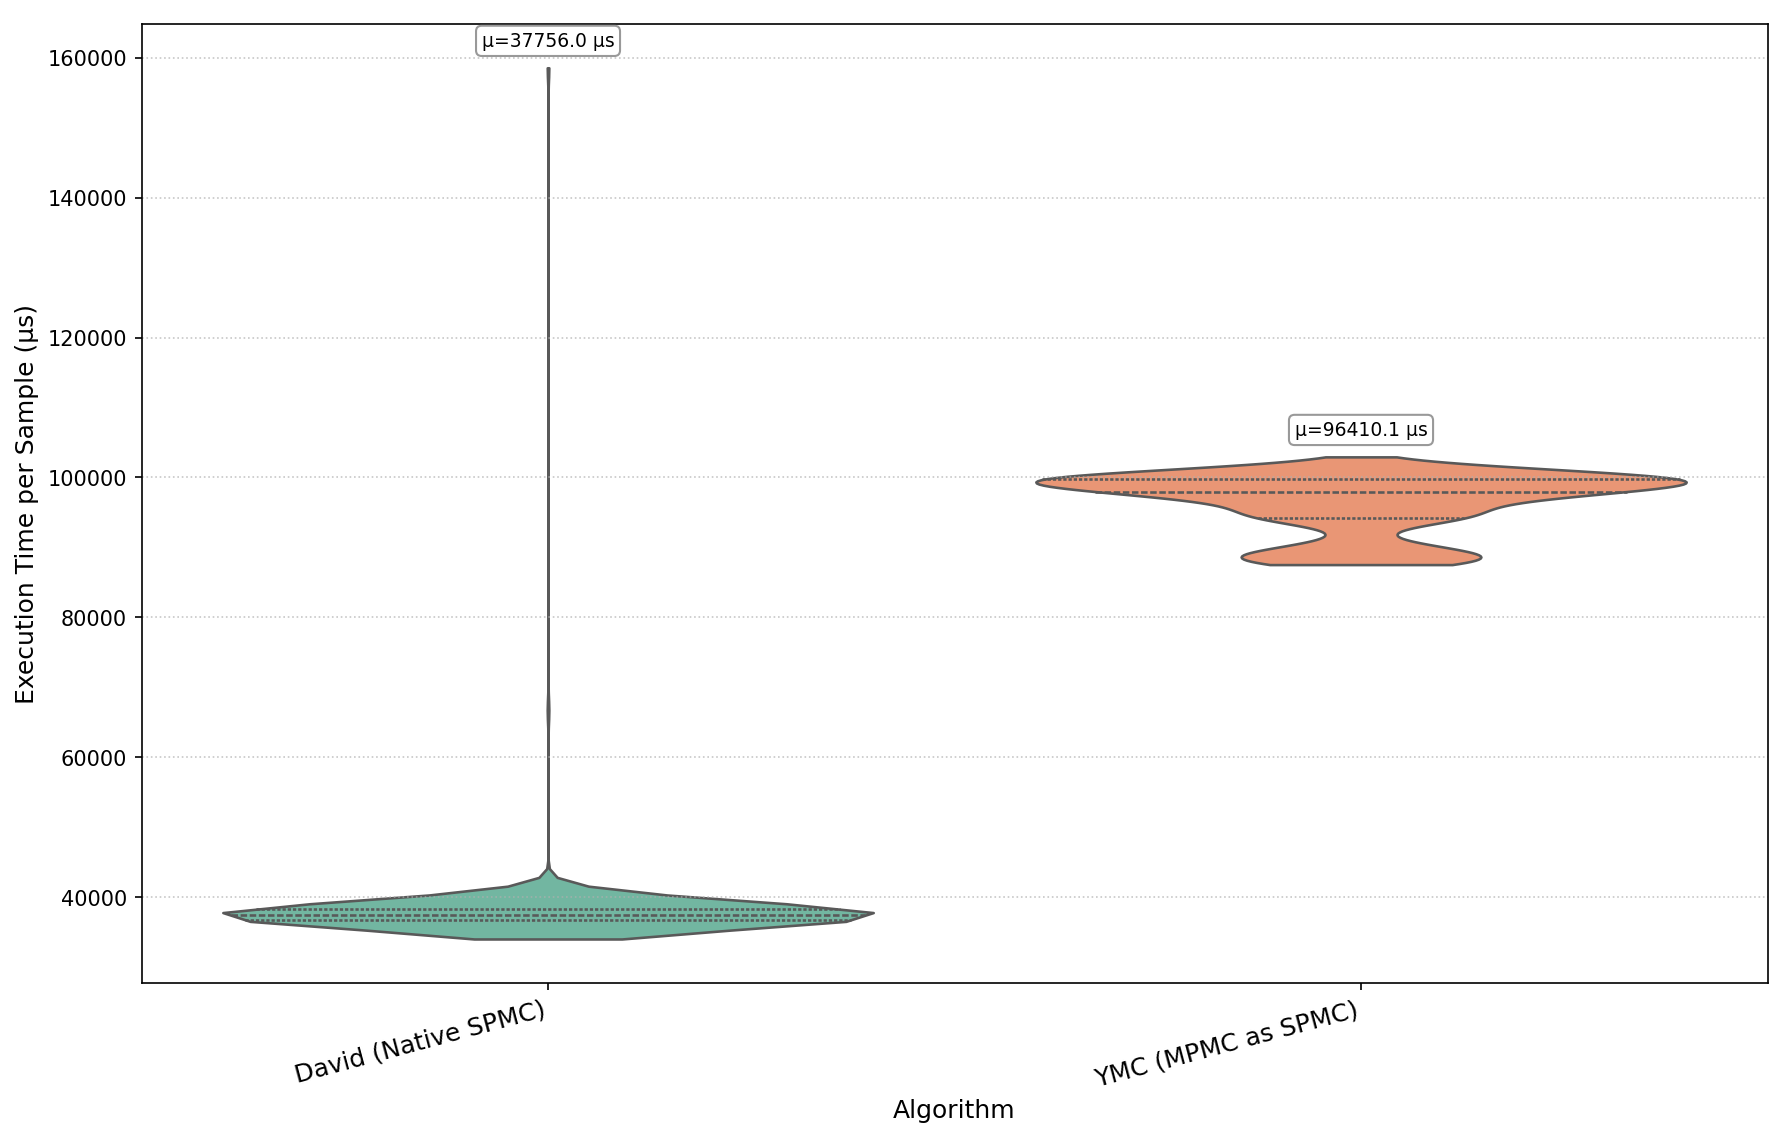
\includegraphics[width=\textwidth]{images/results/best_in_spmc_performance_violin_1P8C.png}
\end{figure}